\providecommand{\main}{../../../..}
\documentclass[\main/dresen_thesis.tex]{subfiles}
  \renewcommand{\thisPath}{\main/chapters/monolayers/structureModel/squareArrayParacrystal}

\begin{document}
  By grazing-incidence small-angle scattering, the in-plane order of a nanostructure is probed over a macroscopic area.
  In this way the structural order of a sample can be quantified using X-rays (GISAXS) and additionally the magnetic order is probed by performing the experiment with neutrons (GISANS).
  The monolayer sample ML-Ac-CoFe-C-2, prepared from the magnetic nanocubes Ac-CoFe-C-2 described in \refapp{app:characterizationAcCoFeC2}, is discussed in the following.
  The GISAS data is described with a paracrystalline square lattice model, which is simulated using the BornAgain software package \cite{Burle_2018_borna}.
  As many parameters enter a GISAS simulation and the simulation is computational expensive, it is important to pre-characterize a sample with complementary experiments first to have a good chance in simulating a model that matches experimental data.

  \begin{figure}[tb]
    \centering
    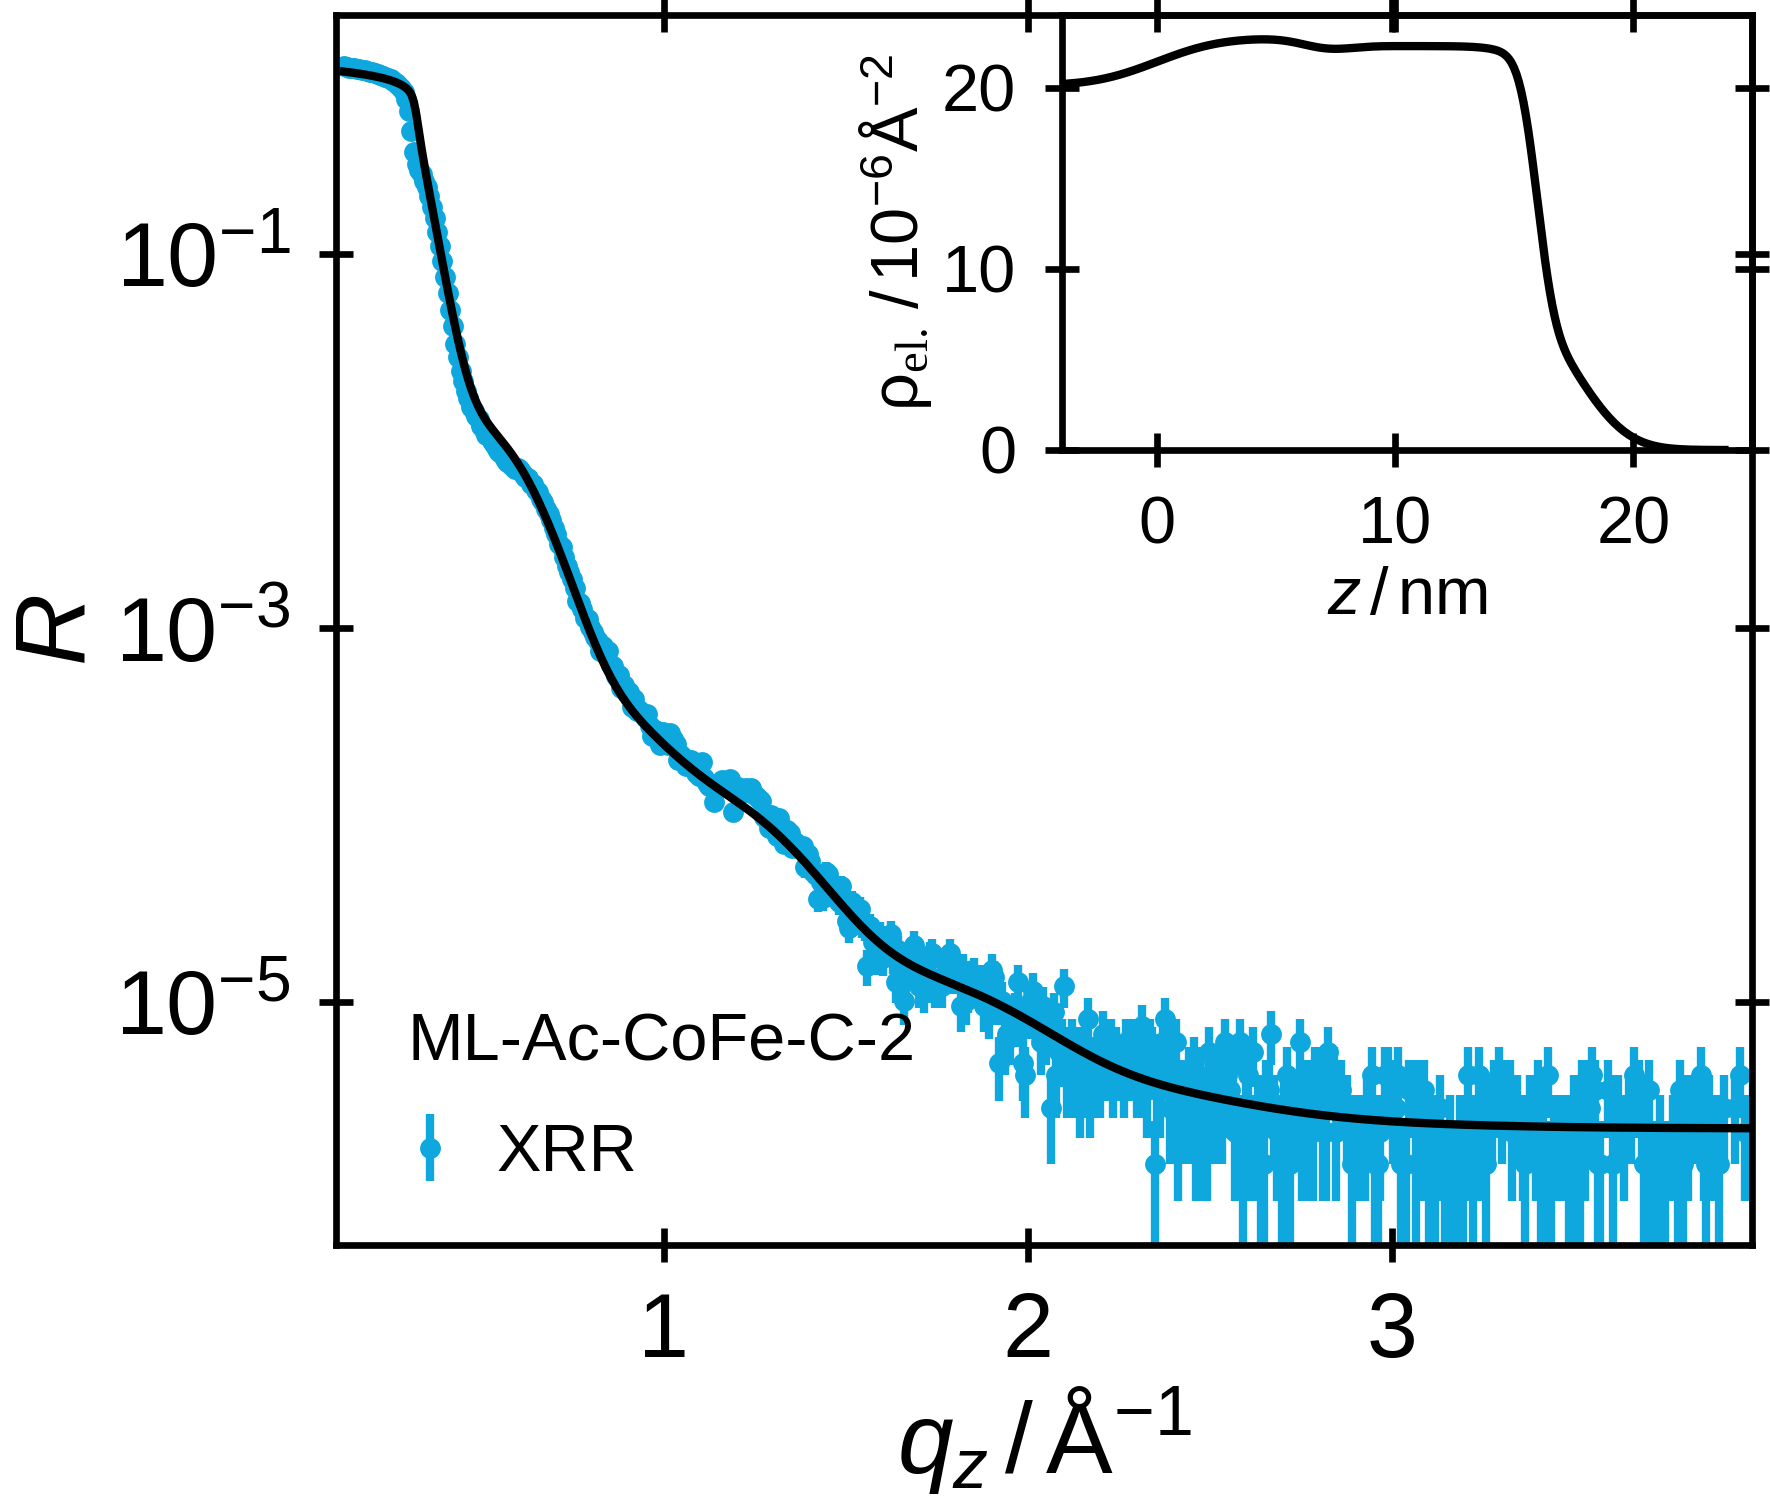
\includegraphics{monolayers_SquareArrayParacrystal_ML_Ac-CoFe-C-2_WithSpacer_XRR}
    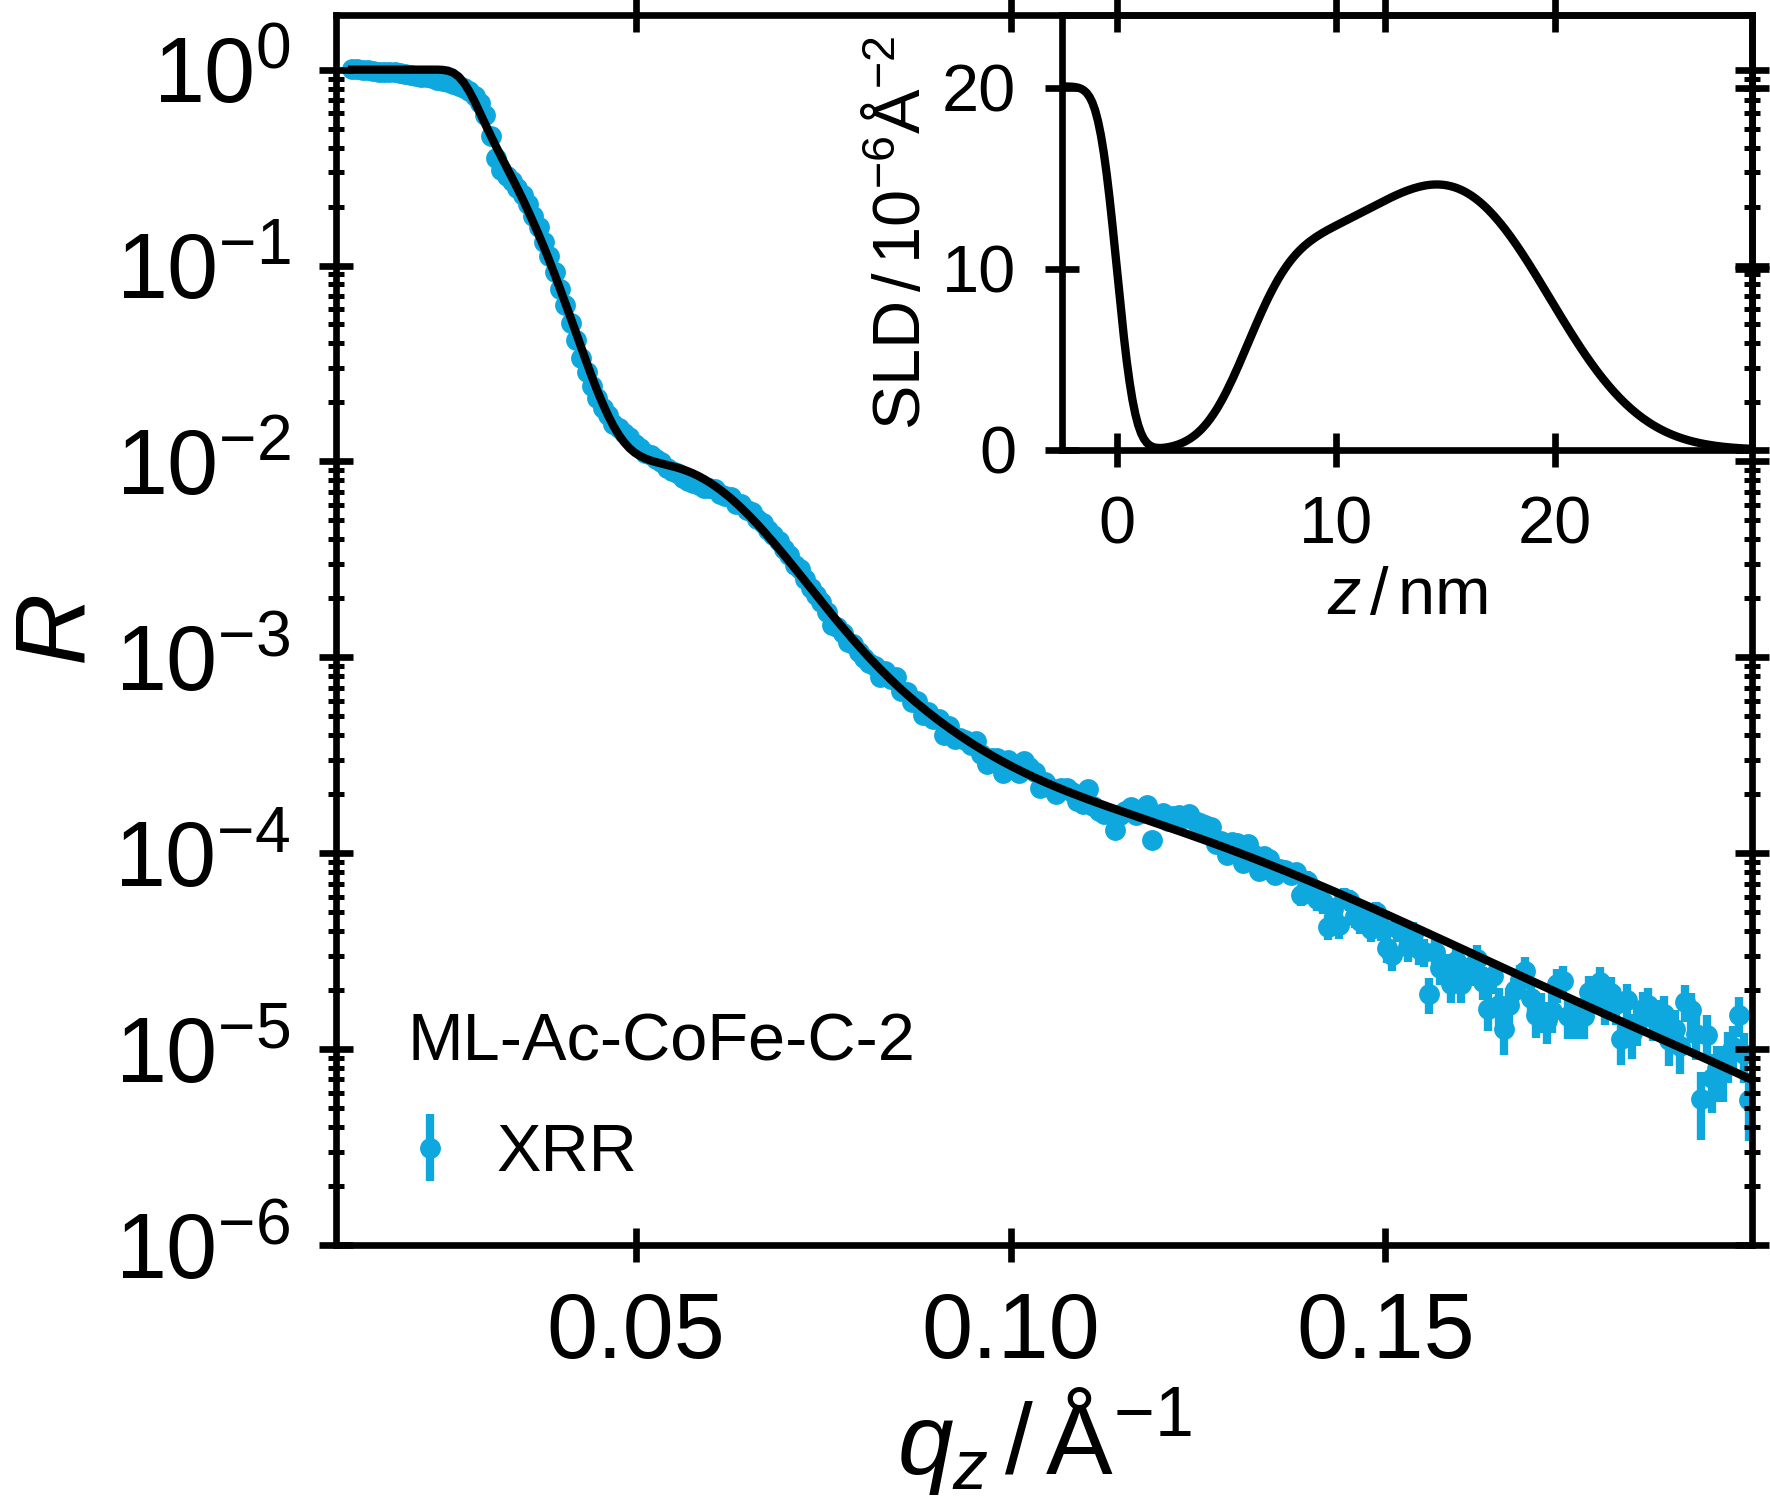
\includegraphics{monolayers_SquareArrayParacrystal_ML_Ac-CoFe-C-2_WithSpacer_FreeSize_XRR}
    \caption{\label{fig:monolayers:structure:squareArrayParacrystal:XRR}XRR of ML-Ac-CoFe-C-2 described according to the model of \refsec{sec:monolayers:structure:verticalModel}. In one case, the particle size is fixed to the value obtained by SAXS (left), in the other the model is free to change at will (right).}
  \end{figure}

  Thus, ML-Ac-CoFe-C-2 is characterized in this section first by XRR, analogue as has been done for the sample ML-Ac-CoFe-C in \refsec{sec:monolayers:structure:verticalModel}.
  Due to the same preparation procedure and as the local structure is comparable to ML-Ac-CoFe-C, which is visible from the SEM micrographs, the same vertical model is used to describe the XRR data.
  However, even though the micrographs suggest a higher quality monolayer, the reflectometry data shows less pronounced peaks in \reffig{fig:monolayers:structure:squareArrayParacrystal:XRR} than in the case of ML-Ac-CoFe-C.
  The reason for the less pronounced peaks is explained by the slightly smaller particle size and the higher size distribution.
  To obtain a decent fit of the model, it is necessary to include the size distribution on the cube layer, which is done by applying a Gauss-Hermite quadrature on the reflectivity intensity, which is described in \refapp{ch:appendix:numericalMethods:sizeDistributions}.
  As the integration is performed over the intensity, the model asserts a locally monodisperse sample, which is reasonable as the self-assembly process in general tends to be size sorting.
  It is again possible to achieve a model that reproduces the main features of the reflectivity curve within the restricted scattering length density profile space that is allowed.
  The \ch{SiO2} and OA layers appear larger than for the previously discussed ML-Ac-CoFe-C, but are still within physically meaningful limits.
  The packing density translates to a mean particle spacing of $14.4(1) \unit{nm}$.

  The agreement of model and data can further be increased by removing the restriction that the mean cube layer thickness is equal to the small-angle X-ray scattering value as done on the right in \reffig{fig:monolayers:structure:squareArrayParacrystal:XRR}.
  This allows the model to scan a larger space of possible scattering length density profiles, but comes with the cost that the parameters have to be reinterpret.
  Parameters of both models are tabulated in \reftab{tab:monolayers:structure:squareArrayParacrystal:XRR}.

  In the result of the second model, the \ch{SiO2} layer represents a low scattering length density layer, taking on the role of the oleic acid layer previously but being a bit thicker and therefore consisting of possibly surplus organic contents that were not removed.
  The originally as oleic acid layer noted layer combines with the original cube layer to an asymmetric profile for the monolayer SLD.
  The particle is therefore the combination of both layers with a thickness of $12.6 \unit{nm}$.
  This larger particle size can be understood as the model trying to simulate a distribution in the particle vertical position, which then after averaging the lateral structure over a large area smears out to an artificially larger particle size.
  Due to this and the small layer thickness size, which is comparable to the roughness in the model, the packing density is also not so straight forward to interpret to a mean particle spacing.
  A particle spacing can however still be estimated from extracting the peak value of the fitted SLD and by comparison with the bulk SLD deduce on the mean packing density.
  This yields for the second model a packing density of $35 \%$, which translates to a particle spacing of $13 \unit{nm}$ when again the SAXS result is used as the true particle size.

  Summarizing the reflectometry results, the careful analysis of multiple models for the data give good estimates for the range of values the parameters are.
  Although the two presented models have some different characteristics, they agree in the existence of a spacer layer between substrate and nanocubes and a mean particle spacing of $13 - 14 \unit{nm}$.
  There is no reason to assume that the vertical model is majorly wrong for the description of the sample and therefore can safely be continued to be used.

  \begin{table}[ht]
    \centering
    \caption{\label{tab:monolayers:structure:squareArrayParacrystal:XRR}Parameters of the models used to describe XRR of ML-Ac-CoFe-C-2 in \reffig{fig:monolayers:structure:squareArrayParacrystal:XRR}.}
    \begin{tabular}{l | c | c}
      \hline
      Model&
      \textbf{Fixed Cube Size} &
      \textbf{Free Cube Size}\\
      \hline
      \multicolumn{3}{c}{\textbf{Particle}}\\
      \hline
      $a \, / \unit{nm}$ &
      $8.58$ &
      $3.9(1)$\\
      $\sigma_a \, / \unit{nm}$ &
        \multicolumn{2}{c}{$15.4 \unit{\%}$} \\
      $\mathrm{SLD}_\mathrm{Cube} \, / \unit{10^{-6} \angstrom^{-2}}$ &
        \multicolumn{2}{c}{$41.749$} \\
      \hline
      \multicolumn{3}{c}{\textbf{Layer}}\\
      \hline
      $\eta_\mathrm{Cube} \, /\, \%$ &
        $43.8(3) $ &
        $62.0(7) $ \\
      $d_{\ch{SiO2}} \, / \unit{nm}$ &
        $7.29(6)$ &
        $6.0(1)$ \\
      $d_{\mathrm{OA, lower}}\, / \unit{nm}$ &
        $5.27(7)$ &
        $8.7(1)$ \\
      $\sigma_{\ch{Si}/\ch{SiO2}} \, / \unit{nm}$ &
        $0.2(1)$ &
        $0.7(1)$ \\
      $\sigma_{\ch{SiO2}/\mathrm{OA}}\, / \unit{nm}$ &
        $2.3(2)$ &
        $1.6(1)$ \\
      $\sigma_\mathrm{OA/Cube} \, / \unit{nm}$ &
        $1.5(1)$ &
        $3.7(1)$ \\
      $\mathrm{SLD}_{\ch{SiO2}} \, / \unit{10^{-6} \angstrom^{-2}}$ &
        $7.8(3)$ &
        $0(1)$\\
      $\mathrm{SLD}_\mathrm{OA} \, / \unit{10^{-6} \angstrom^{-2}}$ &
        $0(1)$ &
        $11.2(2)$ \\
      \hline
      $\mathrm{SLD}_{\ch{Si}} \, / \unit{10^{-6} \angstrom^{-2}}$ &
        \multicolumn{2}{c}{$20.061$} \\
      $d_{\mathrm{OA, upper}}\, / \unit{nm}$ &
        \multicolumn{2}{c}{$0.00$} \\
      \hline
      \multicolumn{3}{c}{\textbf{Instrumental}}\\
      \hline
      $q_\mathrm{shift} \,/ \unit{10^{-3} \angstrom^{-1}}$ &
        $-4.17(5)$ &
        $-4.18(4)$\\
      $\lambda \, / \unit{\angstrom}$ &
        \multicolumn{2}{c}{$1.5418$}\\
      $\Delta \lambda / \lambda\, /\, \%$ &
        \multicolumn{2}{c}{$5.25$} \\
      $I_\mathrm{bg} \, / \unit{10^{-6}}$ &
        \multicolumn{2}{c}{$0.0$} \\
      \hline
    \end{tabular}
  \end{table}

  To investigate the in-plane order, grazing-incidence small-angle scattering is discussed next.
  The experimental data in \reffig{fig:monolayers:structure:ML-Ac-CoFe-C-2:GISAXS} (left) show elongated peaks along $\mathit{q_z}$, which hints to a thin layer structure.
  Furthermore by investigating the Yoneda line along $\mathit{qy}$, the peak positions are analogue to the GISAXS images shown in \refsec{sec:monolayers:preparation:solventProperties}.
  They are describable by two dimensional square lattice indices with only the lattice constant as parameter using \refeq{eq:monolayers:preparation:solventVariation:squareLatticeIndices}.
  The peak position is determined by a Lorentzian fit of the first order peak, yielding $\mathit{q_y}_{10} \eq 0.4733(6) \unit{nm^{-1}}$ and a FWHM of $\gamma \eq 0.053(2) \unit{nm^{-1}}$.
  This translates to a lattice constant of $13.28(2) \unit{nm}$, which is remarkably in between the result obtained by XRR.
  In terms of the paracrystal model \refapp{ch:appendix:calculations:paracrystal}, the FWHM converts to a coherence length of $L_{\mathrm{coh}} \eq 745(28) \unit{nm}$.
  \begin{figure}[tb]
    \centering
    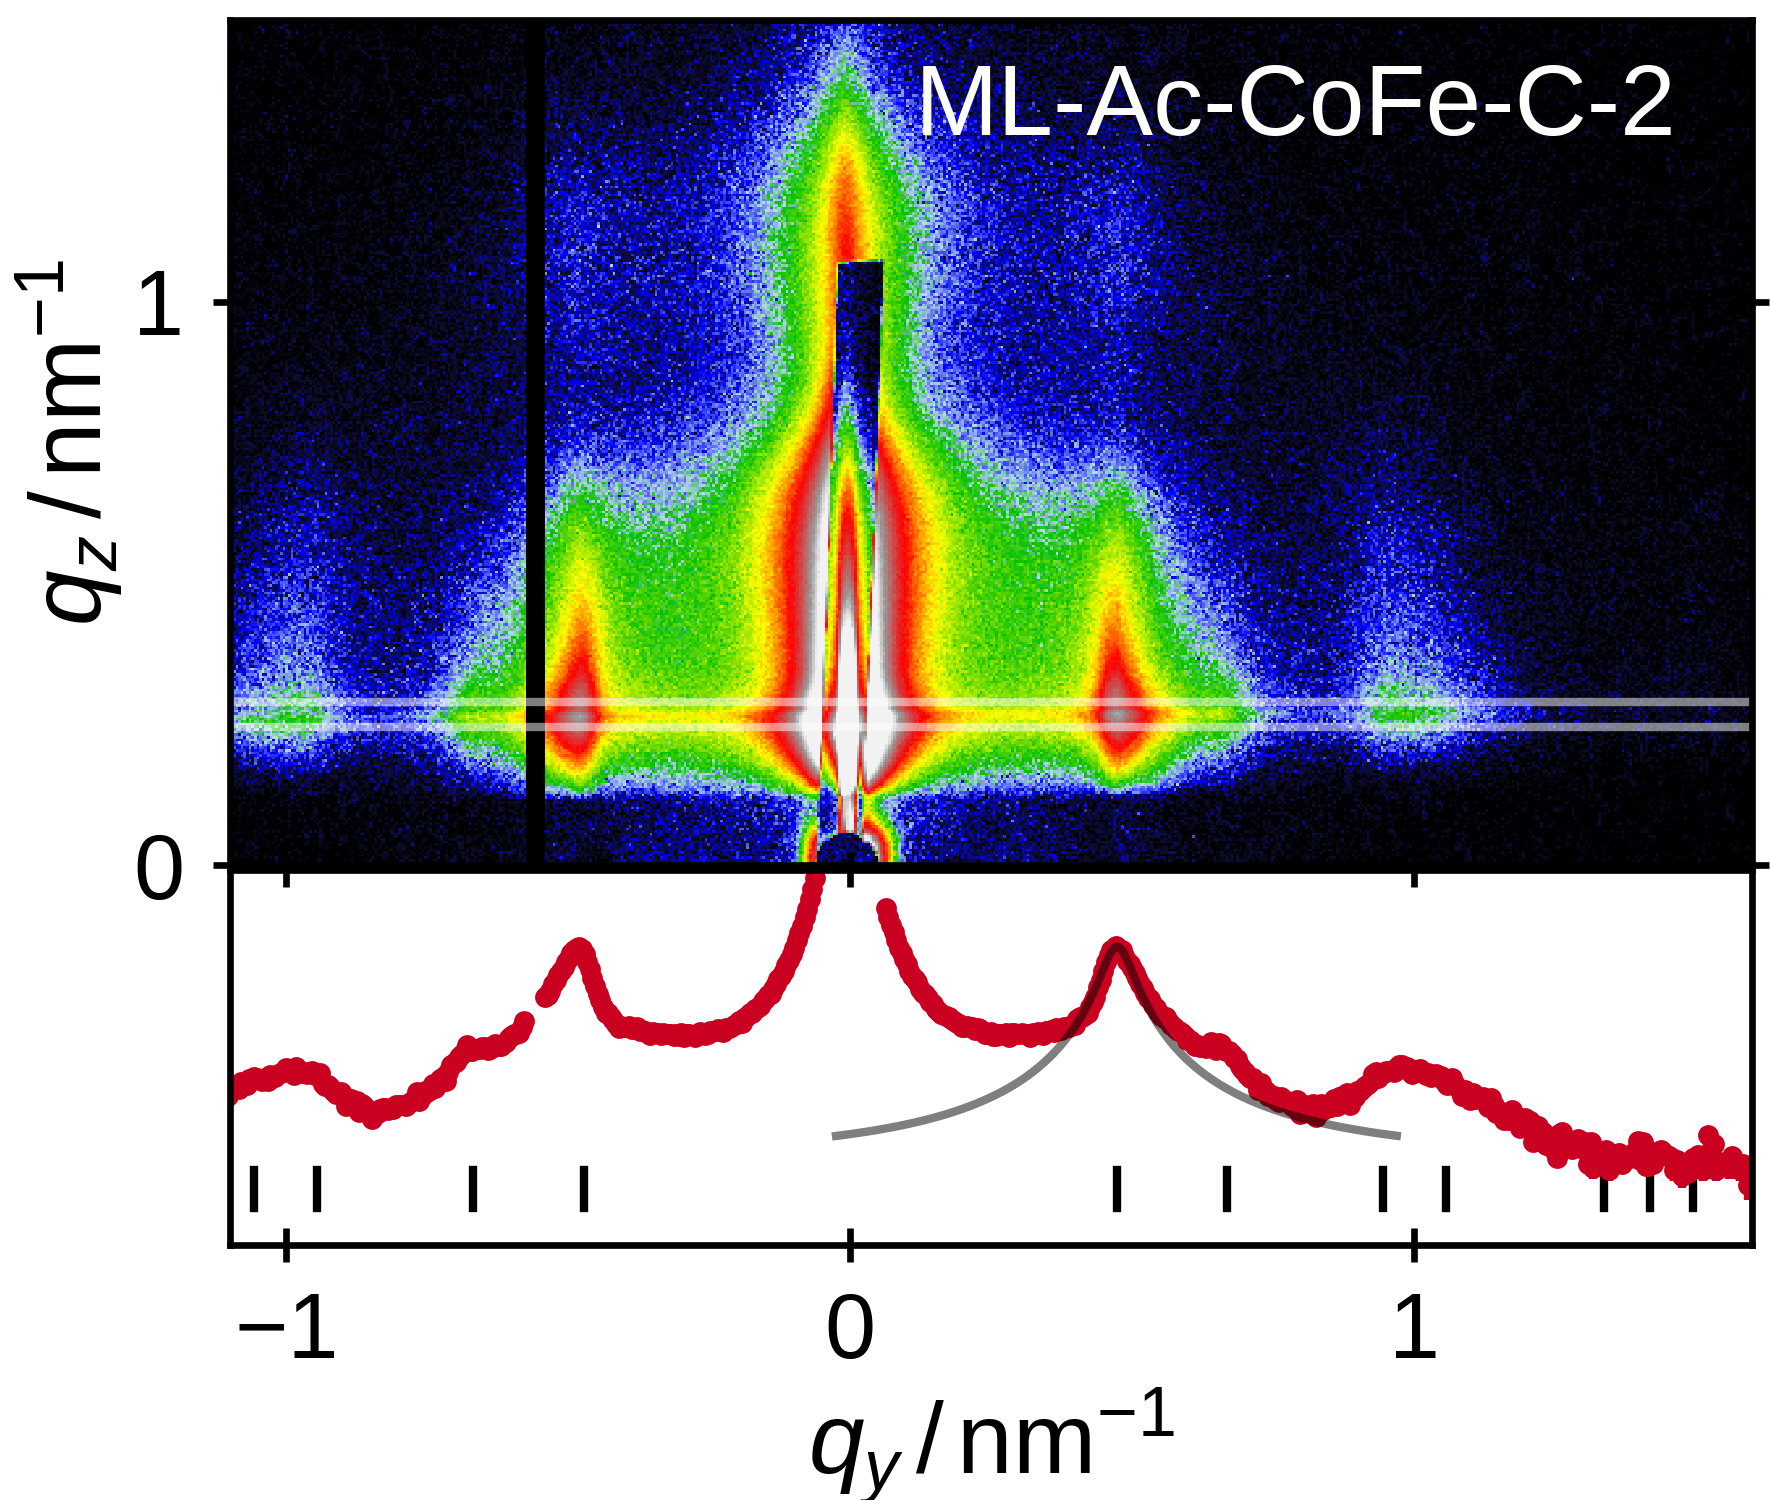
\includegraphics{monolayers_GISAXS_ML-Ac-CoFe-C-2}
    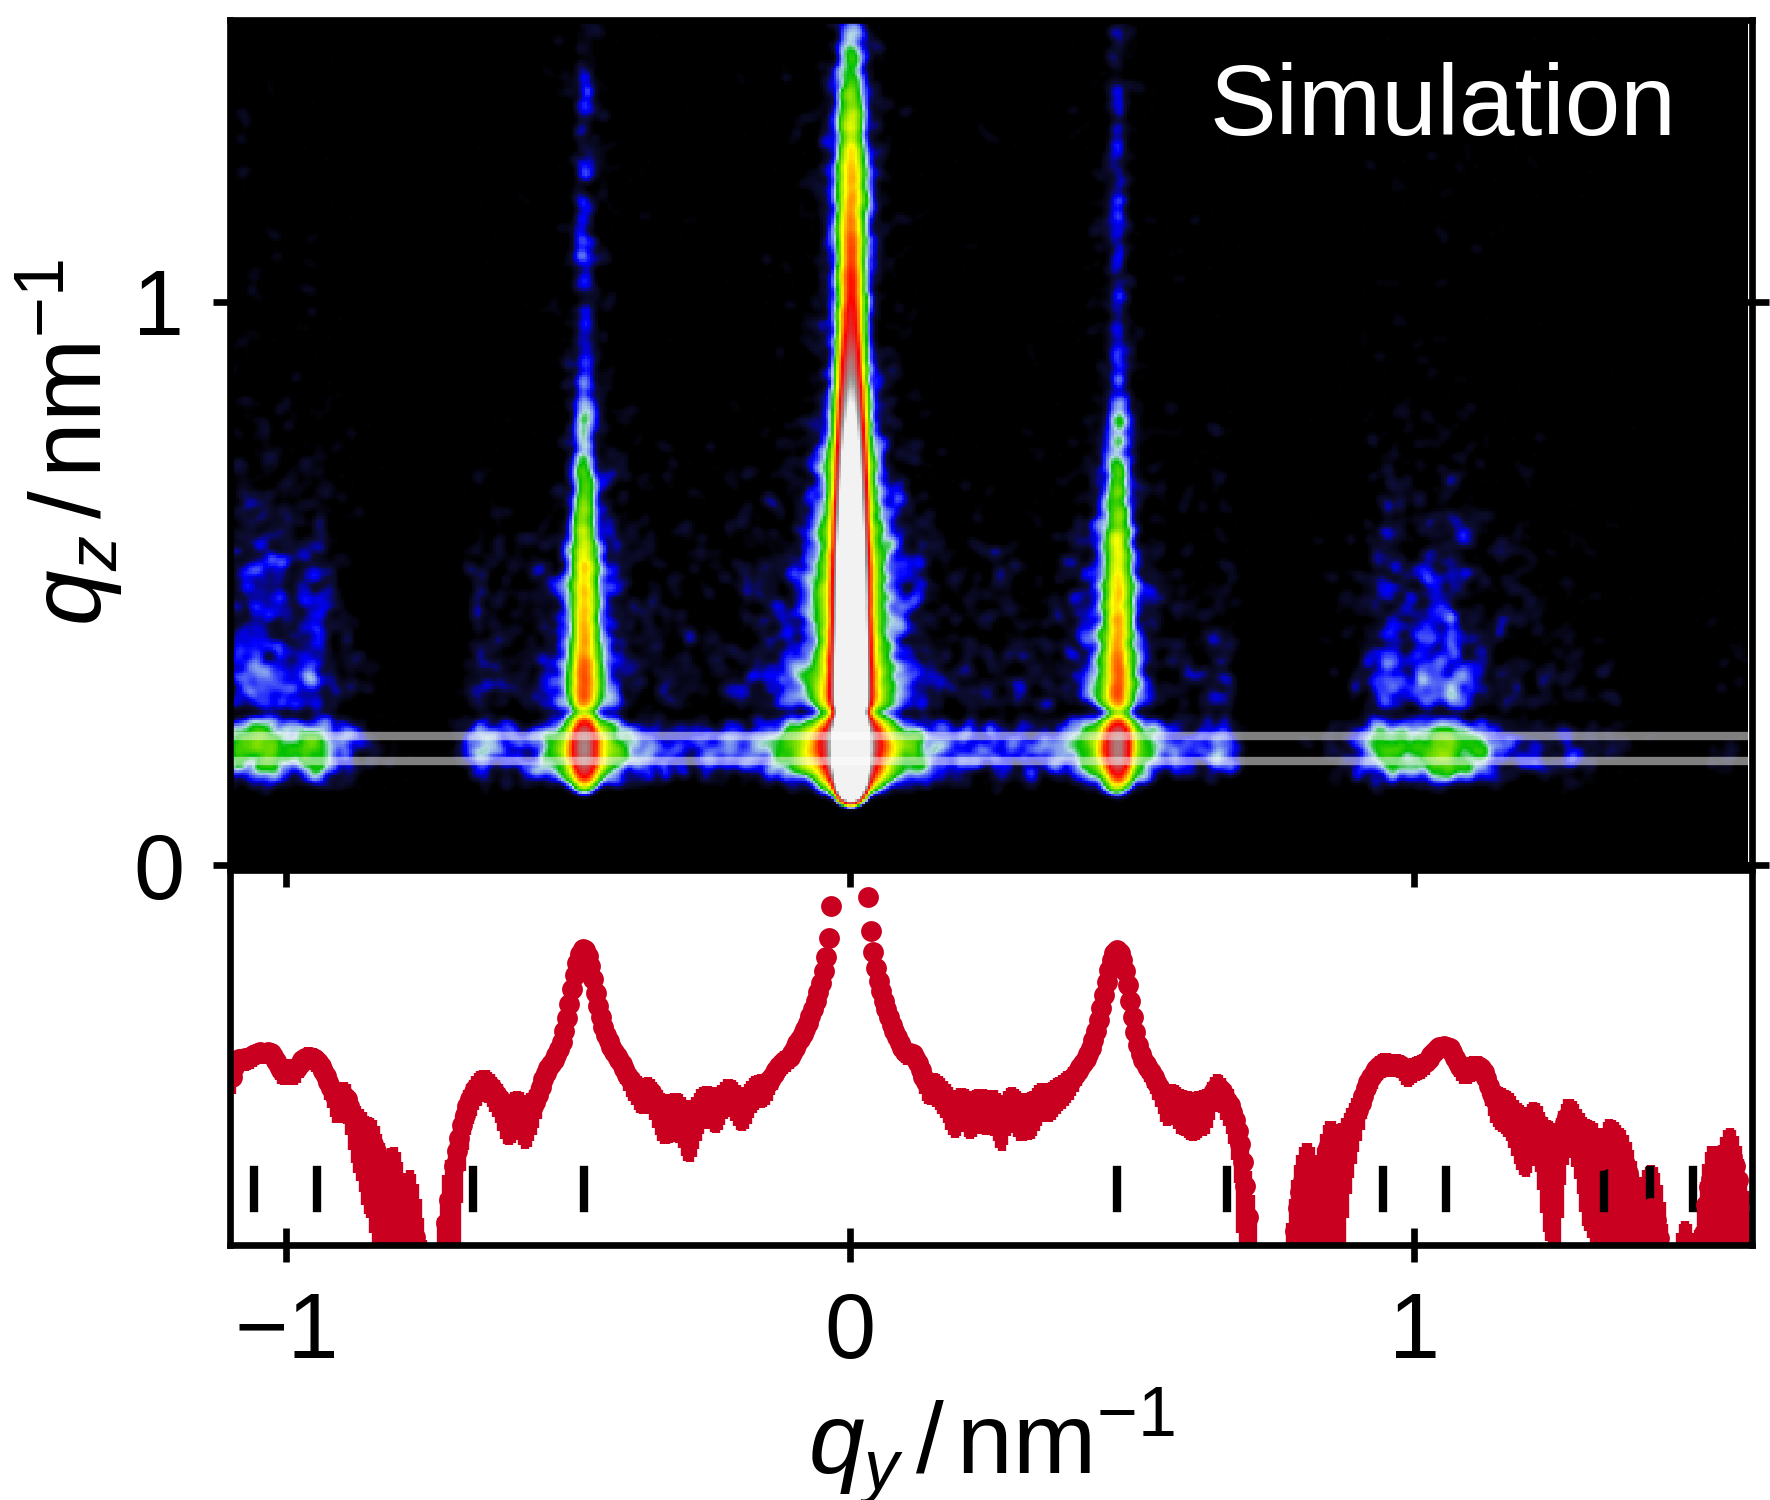
\includegraphics{monolayers_GISAXS_ParacrystalSimulation}
    \caption{\label{fig:monolayers:structure:ML-Ac-CoFe-C-2:GISAXS}GISAXS of ML-Ac-CoFe-C-2 measured at an incident angle of $\alpha_i \eq 0.15$ (left) and simulation of a paracrystal square lattice using the sample properties determined by complimentary experiments (right).}
  \end{figure}

  To verify that the observed GISAXS pattern truly matches with the expectation of a square lattice paracrystal, the software package BornAgain \cite{Burle_2018_borna} is used and the parameters obtained from SAXS, XRR and the Lorentzian fit are entered to describe the sample.
  The GISAXS experiment was performed at the GALAXI instrument and the instrumental parameters as described in \refch{ch:lss:galaxi} are set in the simulation accordingly.
  The structure of the model is depicted in \reffig{fig:monolayers:structure:BornAgainParacrystal}, where the used parameters are listed in \reftab{tab:monolayers:structure:squareArrayParacrystal:BornAgainSimulation} and the simulated result is shown in \reffig{fig:monolayers:structure:ML-Ac-CoFe-C-2:GISAXS} (right).

  \begin{figure}[tb]
    \centering
    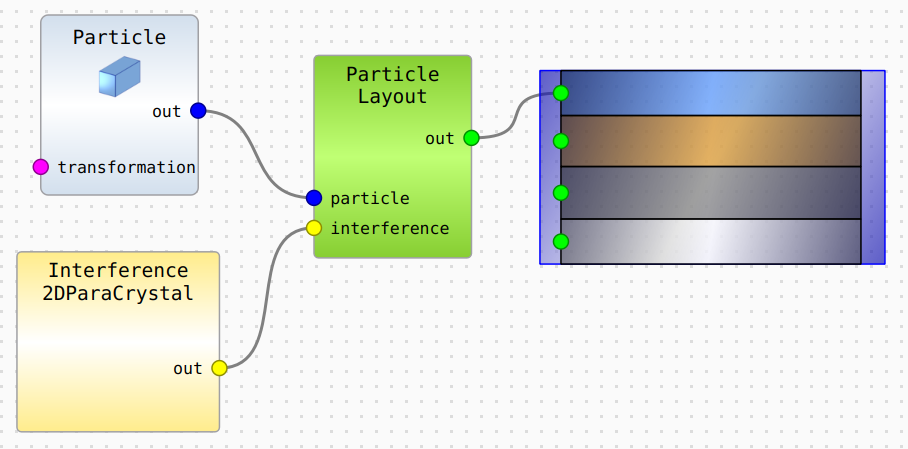
\includegraphics[width=0.9\linewidth]{monolayers_SquareArrayParacrystal_BornAgainParacrystal}
    \caption{\label{fig:monolayers:structure:BornAgainParacrystal}Structure of the square lattice paracrystal model set up in BornAgain.}
  \end{figure}


  \begin{table}[ht]
    \centering
    \caption{\label{tab:monolayers:structure:squareArrayParacrystal:BornAgainSimulation}Square Lattice Paracrystal Model Parameters for the simulation shown in \reffig{fig:monolayers:structure:BornAgainParacrystal}.}
    \begin{tabular}{l | c}
      \hline
      \multicolumn{2}{c}{\textbf{Particle}}\\
      \hline
      $a \, / \unit{nm}$ &
        $8.58$ \\
      $\mathrm{SLD}_\mathrm{Cube} \, / \unit{10^{-6} \angstrom^{-2}}$ &
        $41.75$ \\
      \hline
      \multicolumn{2}{c}{\textbf{Layers}}\\
      \hline
      $d_{\ch{SiO2}}\, / \unit{nm}$ &
        $7.3$\\
      $d_{\mathrm{OA}}\, / \unit{nm}$ &
        $5.3$\\
      $\mathrm{SLD}_{\ch{Si}} \, / \unit{10^{-6} \angstrom^{-2}}$ &
        $20.00$\\
      $\mathrm{SLD}_{\ch{SiO2}} \, / \unit{10^{-6} \angstrom^{-2}}$ &
        $7.78$\\
      $\mathrm{SLD}_\mathrm{OA} \, / \unit{10^{-6} \angstrom^{-2}}$ &
        $0.0$ \\
      \hline
      \multicolumn{2}{c}{\textbf{Paracrystal}}\\
      \hline
      $a_{p-p} \, / \unit{nm}$ &
        $13.275$ \\
      $\sigma_\mathrm{pos.}\, / \unit{nm}$ &
        $0.92$ \\
      $L_\mathrm{damp} \, / \unit{nm}$ &
        $750$ \\
      \hline
      \multicolumn{2}{c}{\textbf{Instrumental}}\\
      \hline
      $\alpha_i \, / \unit{^\circ}$ &
        $0.15$ \\
      $\lambda \, / \unit{\angstrom}$ &
        $1.3414$ \\
      $L_\mathrm{SDD} \, / \unit{mm}$ &
        $1733.5$ \\
      $\Delta q \, /\unit{mm}$ &
        $0.31$ \\
      $I_\mathrm{beam} \, / \unit{10^8}$ &
        $2.5$ \\
      $I_\mathrm{bg}$ &
        Poissonian \\
      \hline
    \end{tabular}
  \end{table}

  Similar to the vertical structure model, it is assumed the sample is a multilayer structure with a \ch{Si} substrate, a \ch{SiO2} intermediate layer and an oleic acid layer, where the nanocubes sit on top.
  For the model parameters, the nanocubes are set to the particle size and SLD as used in SAXS.
  As thickness and scattering length density, the values obtained from the first model in XRR are used.
  As the SLD depends on the X-ray wavelength and the XRR operates at $1.54 \unit{\angstrom}$ while GALAXI operates at $1.34 \unit{\angstrom}$, the values have been rescaled for each material respectively.

  The paracrystalline square lattice interference function uses the lattice constant from the Lorentzian fit.
  For the probability functions of the position uncertainty, Gaussian functions are used. 
  The width of the Gaussian is obtained using \refeq{eq:appendix:calculations:paracrystal:CoherenceLength} and determined to
  \begin{align}
    \sigma_\mathrm{pos.} \eq \sqrt{\frac{a^3}{L_\mathrm{coh}}} \approx 0.92(2) \unit{nm}.
  \end{align}
  As last parameter of the paracrystal model, the damping length, which effectively models a cutoff length for the finite size of a domain, is set to the coherence length.
  As on a large length scale, the square lattice domains are not oriented, the intensity is averaged over all possible two dimensional orientations of the square lattice.
  Particle size distribution and surface roughness of the layers is neglected in this simulation.
  The beam intensity in the BornAgain simulation is chosen such that the signal/noise level is close to the experimental signal/noise ratio.
  After simulation, a rescaling factor is determined from the intensity of the first order peaks to rescale the simulated to the experimental intensity for direct comparison of the patterns.

  The GISAXS data and the BornAgain simulation have the same main features, as to peak positions in the Yoneda linie and detector areas where scattering is visible.
  The experimental data has additionally broader background intensity around the most intense peaks and the first order peak is less elongated along $\mathit{q_z}$ than in the simulation.
  These effects can, however, mostly be attributed to the additional particle size distribution and roughness of the sample.

  In conclusion, the self-consistent agreement between the GISAXS, XRR and SAXS data and the produced model prove that the sample can macroscopically be described by a simple monolayer with paracrystalline long-range order.
  Adding now that the nanocubes are additionally magnetic macrospins, the presented preparation method produces an ideal model system to study dipolar interaction on an ordered two dimensional nanostructure.
\end{document}